\documentclass{beamer}

\mode<presentation> {
	\usetheme{Madrid}
	% \usecolortheme{spruce}   % 浅绿色
	% \setbeamertemplate{navigation symbols}{}  % 隐藏导航符号

	% \setbeamertemplate{footline}
	%若要删除所有幻灯片中的页脚,请取消注释此行
	
	%\setbeamertemplate{footline}[页码]
	%若要用简单的幻灯片计数替换所有幻灯片中的页脚,请取消注释此行
	
	%\setbeamertemplate{导航符号}{}
	%要删除所有幻灯片底部的导航符号,请取消注释此行
}

\usepackage{graphicx} % 允许包含图像
\usepackage{booktabs} % 允许在表中使用\toprule、\ midrule和\ bottomrule
\usepackage[UTF8,noindent]{ctexcap}  % 使用中文输入及显示
\usepackage{gensymb}
\usepackage[bookmarks=true]{hyperref}
\usepackage{tikz}  % 用于图片处理和定位
\usepackage{graphicx}  % 用于插入图片

%-----------------------------------
%	以下为正文
%-----------------------------------

\title[]{2025年迎春杯(小中)数学讲义} 

\author{}
\institute[] % 您的机构将出现在每张幻灯片的底部,可能是节省空间的简写
{
	% 会心升学 \\
	% \medskip
	% \textit{@163.com} % Your email address
}
\date{\today}

\renewcommand{\baselinestretch}{1.3}

\begin{document}
	\begin{frame}
		\vspace{-1cm}
		\begin{flushleft}
			
\includegraphics[width=1cm]{./pics/huixin_logo.png}
		\end{flushleft}
		\titlepage
	\end{frame}

	\begin{frame}
		\frametitle{目录}
		\tableofcontents % 在整个演示过程中,如果您选择使用\ section{}和\ submission{}命令,这些命令将自动打印在此幻灯片上,作为演示的概述
	\end{frame}
	
	%-----------------------------------
	%	开始创建PPT
	%-----------------------------------
	
	% frame counter
	\newcounter{framecounter}
	\section{第1讲\quad 计算}

\item {
    【乘法分配律】
    $(200+2)\times 5 + 5020$ 
    \ifshowSolution
        \fangsong\zihao{4}
        \\
        思路:改。2025

        正解: 
    \else
        \\ \\ \\
    \fi
}

% \item {
%     $(20+2)\times 5 + 2025$ 
%     \ifshowSolution
%         \fangsong\zihao{4}
%         \\
%         思路:2025

%         正解: 
%     \else
%         \\ \\ \\
%     \fi
% }

\item {
    【乘法分配律】
    $7\times 19 + 3\times 13\times 41 + 13\times 19$
    \ifshowSolution
        \fangsong\zihao{4}
        \\
        思路:改。2021;迎春杯四年级真题.pdf

        正解: 
    \else
        \\ \\ \\
    \fi
}

\item {
    【乘法分配律】
    $(18\times 23 - 24\times 17)\div 3 + 5$
    \ifshowSolution
        \fangsong\zihao{4}
        \\
        思路:

        正解: 
    \else
        \\ \\ \\
    \fi
}

\item {
    【乘法分配律】
    $(11\times 24 - 23\times 9)\div 3 + 3$
    \ifshowSolution
        \fangsong\zihao{4}
        \\
        思路:

        正解: 
    \else
        \\ \\ \\
    \fi
}

% \item {
%     【乘法分配律】
%     $7\times 17 + 3\times 13\times 43 + 13\times 17$
%     \ifshowSolution
%         \fangsong\zihao{4}
%         \\
%         思路:2021;迎春杯四年级真题.pdf

%         正解: 2017
%     \else
%         \\ \\ \\
%     \fi
% }

% \item {
%     $(9\times 8\times 7 + 6 - 5)\times 4 + 3 -2 +1$
%     \ifshowSolution
%         \fangsong\zihao{4}
%         \\
%         思路: 迎春杯四年级2022-试卷.pdf

%         正解: 2022
%     \else
%         \\ \\ \\
%     \fi
% }

\item {
    【乘法凑10】
    $12\times 25 + 16\times 15$
    \ifshowSolution
        \fangsong\zihao{4}
        \\
        思路:

        正解: 
    \else
        \\ \\ \\
    \fi
}

\item {
    【乘法凑10】
    $5\times 432\times 1 - 98 - 7\times 6$
    \ifshowSolution
        \fangsong\zihao{4}
        \\
        思路: 2020数学花园探秘笔试小中决赛D卷.doc

        正解: 2020
    \else
        \\ \\ \\
    \fi
}

\item {
    【加法凑10】
    $1+3+4+6+7+9+10 + 12$
    \ifshowSolution
        \fangsong\zihao{4}
        \\
        思路:

        正解: 
    \else
        \\ \\ \\
    \fi
}

\item {
    【乘法凑10】
    $210\times 6 - 52\times 5$
    \ifshowSolution
        \fangsong\zihao{4}
        \\
        思路:

        正解: 
    \else
        \\ \\ \\
    \fi
}

\item {
    【尾同头合十】
    $5000- 22\times 82$  
    \ifshowSolution
        \fangsong\zihao{4}
        \\
        思路:

        正解: 
    \else
        \\ \\ \\
    \fi
}

\item {
    【乘法分配律】
    $67\times 67 - 34\times 34 + 67 + 34$
    \ifshowSolution
        \fangsong\zihao{4}
        \\
        思路:2017年“迎春杯”数学花园探秘科普活动试卷(小中组决赛a卷).doc

        正解: 3434
    \else
        \\ \\ \\
    \fi
}

\item {
    【等差数列求和公式】
    $(1+3+5+\cdots + 89) - (1+2+3+\cdots + 63)$  
    \ifshowSolution
        \fangsong\zihao{4}
        \\
        思路:

        正解: 
    \else
        \\ \\ \\
    \fi
}

\item {
    【数列】
    数列$1, 1,2,3,5,8\cdots$从第二项起每一项都等于它前面两项之和,这个数列成为斐波那契数列.其中每一项都叫做斐波那契数.可以证明“任意正整数n都可以成若干个不同的斐波那契数之和”,那么把100表示成若干个不同的斐波那契数之和有\underline{\hbox to 20mm{}}种表示方法.(只是交换加数的顺序算作同一种)  
    \ifshowSolution
        \fangsong\zihao{4}
        \\
        思路: 2016年“迎春杯”数学花园探秘初赛试卷(四年级b卷).doc

        正解: 9
    \else
        \\ \\ \\
    \fi
}

\item {
    【立方和公式】
    $3^3 + 4^3 + 5^3 + 6^3 + 7^3 + 8^3 + 9^3$
    \ifshowSolution
        \fangsong\zihao{4}
        \\
        思路:

        正解: 
    \else
        \\ \\ \\
    \fi
}

\item {
    【数值计算】
    $99\times 10101\times 111\times 1001001$的末5位数字是多少?
    \ifshowSolution
        \fangsong\zihao{4}
        \\
        思路:

        正解: 88889
    \else
        \\ \\ \\
    \fi
}

\item {
    【数值计算;数字谜】
    正着读和反着读都一样的数称为回文数,如121、9889都是回文数,如果一个三位回文数和一个四位回文数的和是 2025,那么这两个回文数的差是\underline{\hbox to 20mm{}}.
    \ifshowSolution
        \fangsong\zihao{4}
        \\
        思路: 综合-数字谜.

        正解: 改  2023;YCB第40届小中组试卷.pdf; 1551+474=2025
    \else
        \\ \\ \\
    \fi
}

\item {
    【数值计算;数字谜】有一些自然数,如 121 和 2552,从左到右和从右到左的数字顺序相同,我们把这样的自然数叫做``回文数''. 已知两个回文数的和是 2022,则这两个回文数的差是\underline{\hbox to 20mm{}}.
    \ifshowSolution
        \fangsong\zihao{4}
        \\
        思路: 综合-数字谜.

        正解:  迎春杯三年级2022-试卷.pdf; 1740
    \else
        \\ \\ \\
    \fi
}

% \item {
%     【数字谜】
%     下列竖式中,相同汉字表示相同数字,不同汉字表示不同数字,且所有汉字对应的数字都不是 0,2,5。 ``空歌风度清'' 表示的五位数是\underline{\hbox to 20mm{}}.
%     \zihao{2}
%     \begin{figure}[H] 
%         \centering
%         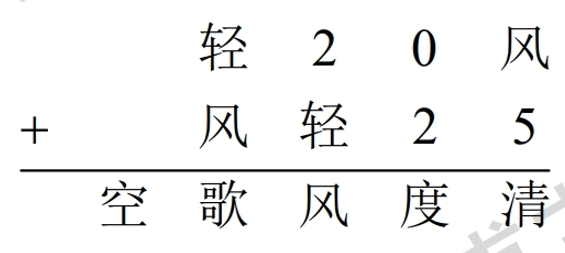
\includegraphics[width=0.4\textwidth]{./pics/Chapter_7/1.png}
%     \end{figure}
%     \vspace{1cm}
%     % 2025数学花园探秘笔试小中年级决赛C卷(B5试卷版).pdf;16934
% }

\item {
    【数字谜】
    下面的算式中,相同的汉字代表相同的数字,不同的汉字代表不同的数字,那么,\\ \myoverline{龙行天下}  表示的四位数是\underline{\hbox to 20mm{}}.
    \begin{figure}[H] 
        \centering
        
\includegraphics[width=0.4\textwidth]{./pics/Chapter_7/2.png}
    \end{figure}
    \vspace{1cm}
    % 2024
}

\item {
    【数字谜】
    将 $1\sim 9$分别填入到右图的方框中,每个数字用一次,使得竖式成立;现在数字 6、7、8已经被填入,那么竖式的和是\underline{\hbox to 20mm{}}.
    \zihao{2}
    \[
    \begin{array}{r@{\,}r@{}c@{}l}
    & \square & \square & \square \\
    + & \square  & \boxed{7} & \boxed{6} \\
    \cline{1-4}
    & \boxed{8} & \square & \square \\
    \end{array}
    \]
    % \begin{figure}[H] 
    %     \centering
    %     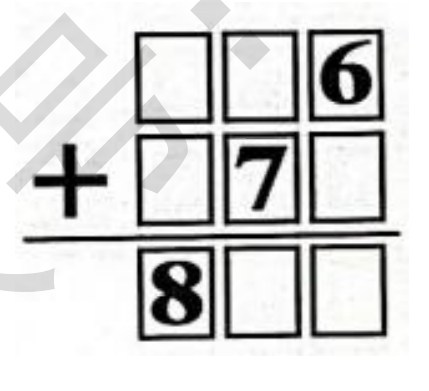
\includegraphics[width=0.3\textwidth]{./pics/Chapter_7/3.png}
    % \end{figure}
    \vspace{1cm}
    % 2023YCB初赛真题答案小中.pdf; 819
    % 改
}

\item {
    【数字谜】
    在右图的加法竖式中,6个汉字恰好代表6个连续的数字,那么,``花园探秘'' 所代表的四位数是\underline{\hbox to 20mm{}}.
    \begin{figure}[H] 
        \centering
        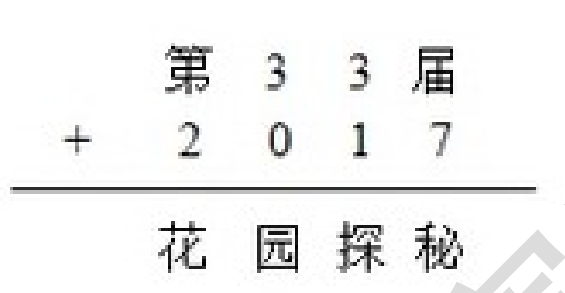
\includegraphics[width=0.4\textwidth]{./pics/Chapter_7/12.png}
    \end{figure}
    \vspace{1cm}
    % 2021; 8354
}

\item {
    【数字谜】
    在右面的乘法竖式中,相同的汉字代表相同的数字,不同的汉字代表不同的数字;那么,\myoverline{迎接夏天} 代表的四位数是\underline{\hbox to 20mm{}}.
    \begin{figure}[H] 
        \centering
        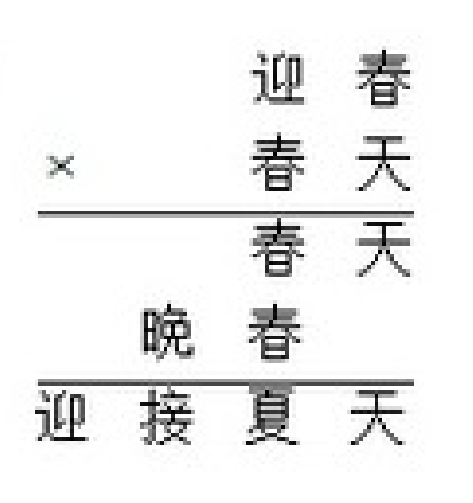
\includegraphics[width=0.4\textwidth]{./pics/Chapter_7/14.png}
    \end{figure}
    \vspace{1cm}
    % 2021,迎春杯四年级真题.pdf; 1024
}
	\section{数论}

\title[第2讲\quad 数论]{第2讲\quad 数论} 
\author{}
\date{}

\begin{frame}
    \titlepage
\end{frame}

\setcounter{framecounter}{0}

\begin{frame}
    \stepcounter{framecounter}
    \frametitle{习题\theframecounter}
    \vspace*{-3cm}
    \center\textit{再过12天就到2016年了,昊昊感慨地说:我到目前只经过2个闰年,并且我出生的年份是9的倍数,那么2016年昊昊是 \underline{\hbox to 20mm{}} 岁.} 
    % 9
\end{frame}

\begin{frame}
    \stepcounter{framecounter}
    \frametitle{习题\theframecounter}
    \vspace*{-3cm}
    \textit{一个整数减去 77,然后乘以 8,再除以 7,所得的商是 37,而且有余数。这个数是多少?} 
    % 110
\end{frame}

\begin{frame}
    \stepcounter{framecounter}
    \frametitle{习题\theframecounter}
    \vspace*{-3cm}
    \textit{王老师在一个特殊的学校上课,他每上3天课可以休息一天,已知本学期他第一次休息在星期二,那么他第五次休息是星期\underline{\hbox to 20mm{}} (填数字1--7).} % 4
\end{frame}

\begin{frame}
    \stepcounter{framecounter}
    \frametitle{习题\theframecounter}
    \vspace*{-3cm}
    \textit{今天是1月30日,我们先写下130;后面写数的规则是:如果刚写下的数是偶数就把它除以2再加上2写在后面,如果刚写下的数是奇数就把它乘以2再减去2写在后面,于是得到:130、67、132、68…,那么这列数中第2016个数是\underline{\hbox to 20mm{}}} % 6
\end{frame}

\begin{frame}
    \stepcounter{framecounter}
    \frametitle{习题\theframecounter}
    \vspace*{-3cm}
    \textit{一组有两位数组成的偶数项等差数列,所有奇数项的和为100,若从第1项开始,将每个奇数项与它后面相邻的偶数项不改变次序地合并成一个四位数,形成一个新的数列,那么新数列的和与原数列的和相差\underline{\hbox to 20mm{}}.} % 9900
\end{frame}

\begin{frame}
    \stepcounter{framecounter}
    \frametitle{习题\theframecounter}
    \vspace*{-3cm}
    \textit{现在有一台奇怪的电脑,电脑上有个按键,如果电脑上原来的数是3的倍数,按下键后就会除以3;如果电脑上原来的数不是3的倍数,那么按下键后就会乘以6.小明在按键前没有看屏幕上的数,结果连按6次,最后电脑上显示的数是12,那么电脑上最开始的数最小可能是\underline{\hbox to 20mm{}}.} % 27
\end{frame}

\begin{frame}
    \stepcounter{framecounter}
    \frametitle{习题\theframecounter}
    \vspace*{-3cm}
    \textit{有一些自然数,如 121 和 2552,从左到右和从右到左的数字顺序相同,我们把这样的自然数叫做“回文数”.已知两个回文数的和是 2022,则这两个回文数的差是\underline{\hbox to 20mm{}}.} 
    % 2022; 
\end{frame}

\begin{frame}
    \stepcounter{framecounter}
    \frametitle{习题\theframecounter}
    \vspace*{-3cm}
    \textit{$99\times 10101\times 111\times 1001001$的末5位数字是多少?} % 88889
\end{frame}

\begin{frame}
    \stepcounter{framecounter}
    \frametitle{习题\theframecounter}
    \vspace*{-3cm}
    \textit{已知 $S = 2^{2020} + 3^{2021} + 4^{2022} + 5^{2023} +6^{2024} + 7^{2025}$, 则 $S$ 的末位数字是多少?} % 3
\end{frame}

\begin{frame}
    \stepcounter{framecounter}
    \frametitle{习题\theframecounter}
    \vspace*{-3cm}
    \textit{数列 $121, 1221, 12221, 122221,\cdots$ 的前2025项中,有多少项能被3整除?} % 675
\end{frame}

\begin{frame}
    \stepcounter{framecounter}
    \frametitle{习题\theframecounter}
    \vspace*{-3cm}
    \textit{有一个数除以3余 2,除以4余 1. 此数除以 12 余\underline{\hbox to 20mm{}}.} % 5
\end{frame}

\begin{frame}
    \stepcounter{framecounter}
    \frametitle{习题\theframecounter}
    \vspace*{-3cm}
    \textit{各位数字都是 7,并能被 63 整除的最小自然数是\underline{\hbox to 20mm{}}.} % 777777777
\end{frame}

\begin{frame}
    \stepcounter{framecounter}
    \frametitle{习题\theframecounter}
    \vspace*{-3cm}
    \textit{一个三位数被 3 除余 1,被 5 除余 3,被 7 除余 5,这个数最大是\underline{\hbox to 20mm{}}.} % 943
\end{frame}

\begin{frame}
    \stepcounter{framecounter}
    \frametitle{习题\theframecounter}
    \vspace*{-3cm}
    \textit{一个整数减去 77,然后乘以 8,再除以 7,所得的商是 37,而且有余数。这个数是 \underline{\hbox to 20mm{}}.} % 110
\end{frame}

\begin{frame}
    \stepcounter{framecounter}
    \frametitle{习题\theframecounter}
    \vspace*{-3cm}
    \textit{已知被除数比除数大 80,并且商是 8,余数是 3,则被除数与除数之积是 \underline{\hbox to 20mm{}}.} % 1001
\end{frame}

\begin{frame}
    \stepcounter{framecounter}
    \frametitle{习题\theframecounter}
    \vspace*{-3cm}
    \textit{已知 $A$ 是一个两位数,$A^2$ 除以15的余数为1,则满足条件的 $A$ 的个数为 \underline{\hbox to 20mm{}}.} 
    % 华数真题2021-2023(小中组).pdf;24
\end{frame}

	\section{第3讲\quad 几何}

\item {
    在长方形$ABCD$中, $P,Q$分别是$AD,BC$的中点, $EM\mathop{//}NF\mathop{//}AD$, $AE=CF=6$,影部分面积为51, 那么$AD$的长度为\underline{\hbox to 20mm{}}.
    \begin{figure}[H] 
        \centering
        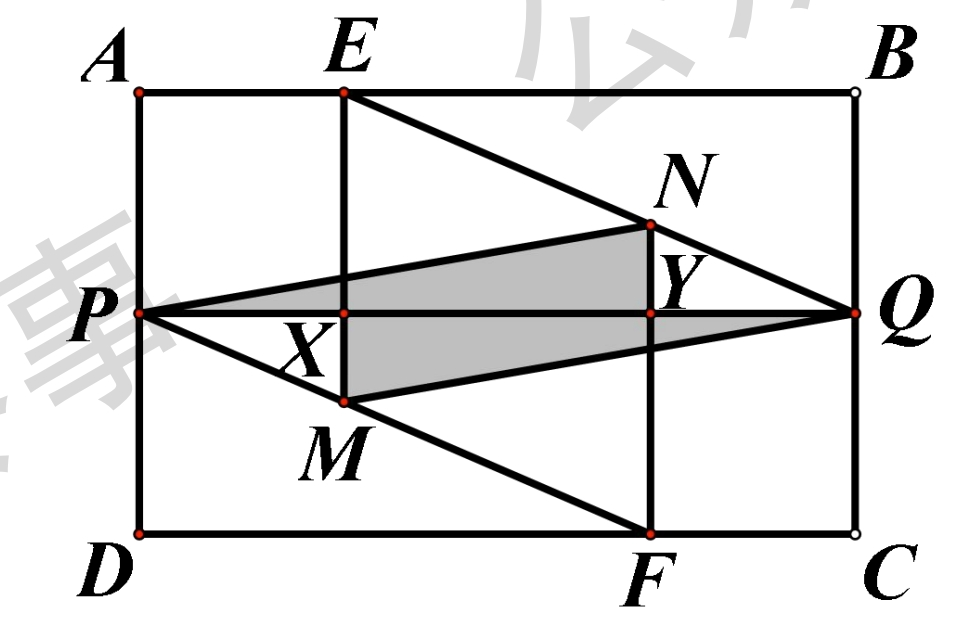
\includegraphics[width=0.4\textwidth]{./pics/Chapter_3/1.png}
    \end{figure}
    \vspace{1cm}
    % 17
}

\item {
    如图,边长为24的大正方形被分成了五个周长相等的长方形,那么阴影长方形的面积是 \underline{\hbox to 20mm{}}.
    \begin{figure}[H] 
        \centering
        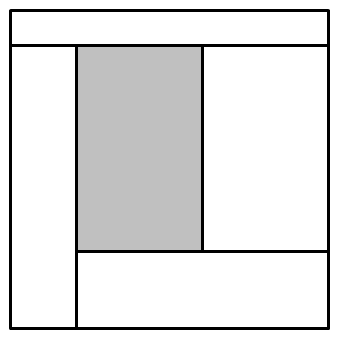
\includegraphics[width=0.2\textwidth]{./pics/Chapter_3/2.png}
    \end{figure}
    \vspace{1cm}
    % 
}

\item {
    如图,正六边形ABCDEF中,以AB为边长向内作正方形ABGH,CG与FH交于点M.\\
    (1)如果正六边形ABCDEF的边长是20,那么三角形AFH的面积是\underline{\hbox to 20mm{}}.\\
    (2)如果正六边形ABCDEF的面积是24,那么阴影部分面积之和是\underline{\hbox to 20mm{}}.
    \begin{figure}[H] 
        \centering
        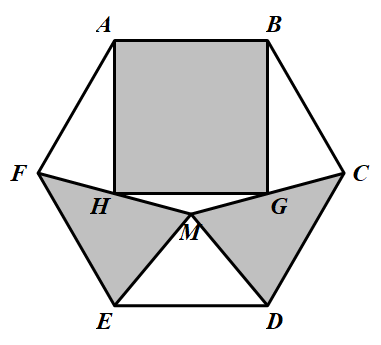
\includegraphics[width=0.4\textwidth]{./pics/Chapter_3/3.png}
    \end{figure}
    \vspace{1cm}
    % 
}
\item {
    如图,一个大正方形被分割成了周长依次为70、80、90、100的四个小长方形;那么,其中最小的小长方形的面积是\underline{\hbox to 20mm{}}.
    \begin{figure}[H] 
        \centering
        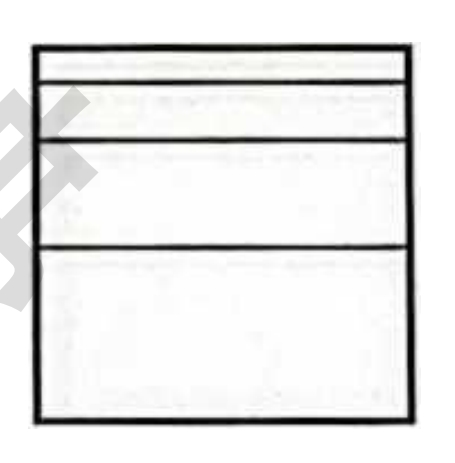
\includegraphics[width=0.2\textwidth]{./pics/Chapter_3/4.png}
    \end{figure}
    \vspace{1cm}
    % 
}

\item {
    {两个完全一样的长方形如图摆放,如果整个图形的面积是 420平方厘米,那么阴影部分的面积是\underline{\hbox to 20mm{}}平方厘米.} 
    \begin{figure}[H] 
        \centering
        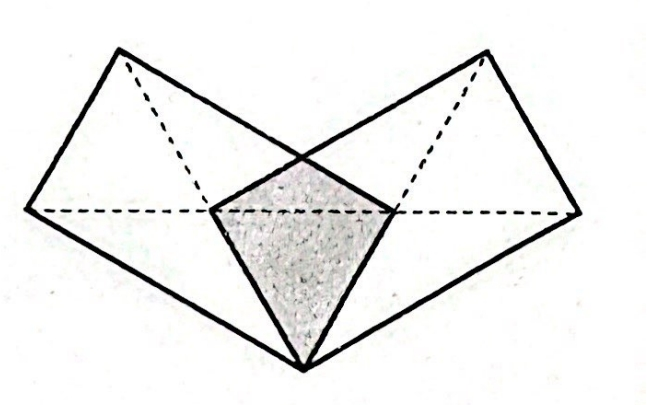
\includegraphics[width=0.4\textwidth]{./pics/Chapter_3/5.png}
    \end{figure}
    \vspace{1cm}
    % 84
}
\item {
    {在一个长方形纸片的左下角剪掉一个小长方形,
    再切成三块, 这三块恰好可以拼成一个三角形,
    若长方形的宽为12, AB的长度是CD的5倍,
    那么EC的长度为\underline{\hbox to 20mm{}}.} 
    \begin{figure}[H] 
        \centering
        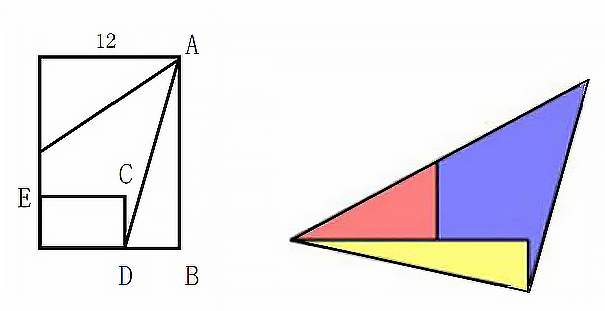
\includegraphics[width=0.6\textwidth]{./pics/Chapter_3/6.png}
    \end{figure}
    \vspace{1cm}
    % 
}

\item {
    {如图所示,一个正五边形与两个正六边形相邻,它们的边长相等。则$\angle ABC = $\underline{\hbox to 20mm{}}.} 
    \begin{figure}[H] 
        \centering
        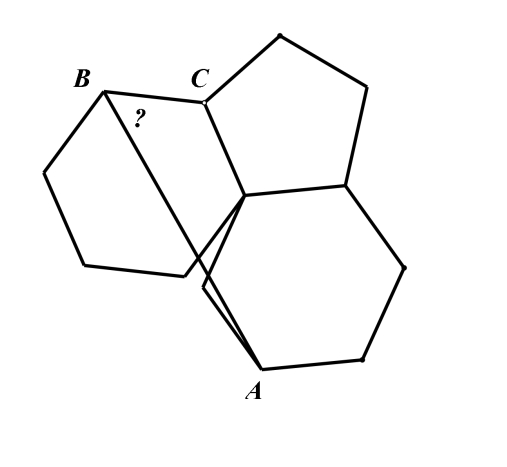
\includegraphics[width=0.4\textwidth]{./pics/Chapter_3/7.png}
    \end{figure}
    \vspace{1cm}
    % 华杯202103
}
\item {
    {如图,三角形 ABC和三角形 ADE是 $\angle A=90\degree$ 的等腰直角三角形,点 M 是 BC 的中点。已知$AB=AC=DF=FM=EG=GM$, $\angle FDE = \angle GED=9\degree$ 且点F和点G在三角形ADE以外. 问$\angle FMG$ 的度数是( )度.} 
    \begin{figure}[H] 
        \centering
        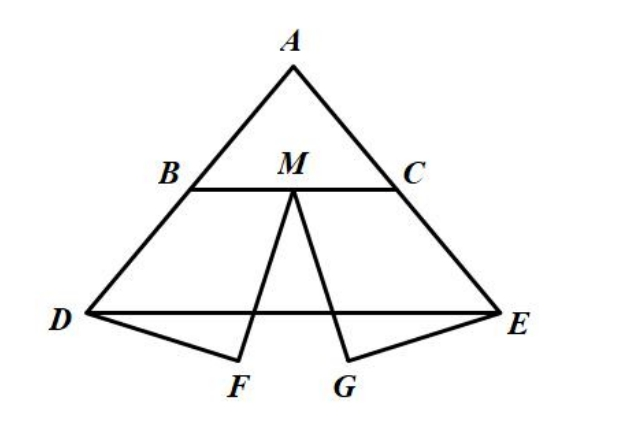
\includegraphics[width=0.4\textwidth]{./pics/Chapter_3/8.png}
    \end{figure}
    \vspace{1cm}
    % 华数真题2021-2023(小中组).pdf, 2022.2.19线上小中组解析1.pdf; 54
}

\item {
    {在下图中,$\angle 1 + \angle 2 + \angle 3 + \angle 4 - \angle 5=$ \underline{\hbox to 20mm{}} $\degree$.} 
    \begin{figure}[H] 
        \centering
        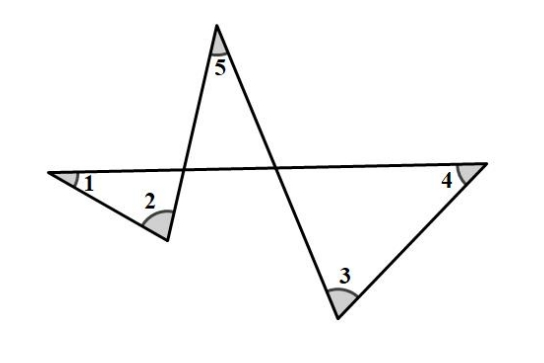
\includegraphics[width=0.4\textwidth]{./pics/Chapter_3/9.png}
    \end{figure}
    \vspace{1cm}
    % 华数真题2021-2023(小中组).pdf
}
\item {
    {如图所示,一个正方形纸片ABCD沿对角线BD剪成两个三角形.第一步操作,将三角形ABD竖直向下平移3厘米至三角形EFG;第二步操作,将三角形EFG竖直向下再平移5厘米至三角形HIJ.第一步操作后两张纸片重叠的面积与第二步操作后两张纸片重叠的面积相等,那么这个正方形纸片ABCD的面积是 \underline{\hbox to 10mm{}} 平方厘米.} 
    \begin{figure}[H] 
        \centering
        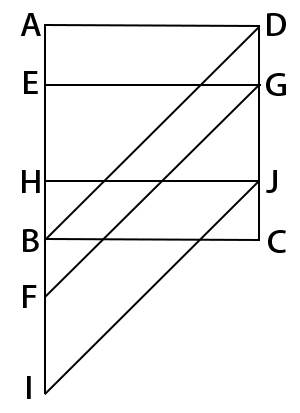
\includegraphics[width=0.2\textwidth]{./pics/Chapter_3/10.png}
    \end{figure}
    \vspace{1cm}
    % 2018年第二十三届“华罗庚金杯”少年数学邀请赛初赛试卷(小中组).doc; 121
}

\item {
    {从四边形4个内角取2个求和,共有6个和数,则大于180°的和最多有 \underline{\hbox to 20mm{}} 个.} 
    \begin{figure}[H] 
        \centering
        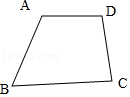
\includegraphics[width=0.2\textwidth]{./pics/Chapter_3/11.png}
    \end{figure}
    \vspace{1cm}
    % 华杯2018; 3
}
\item {
    {如图,将一个正方形硬纸片的四个角分别剪去一个等腰直角三角形,最后剩下一个长方形.正方形边长和三角形直角边长都是整数.若剪去部分的总面积为40平方厘米,则长方形的面积是 \underline{\hbox to 20mm{}} 平方厘米.} 
    \begin{figure}[H] 
        \centering
        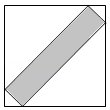
\includegraphics[width=0.2\textwidth]{./pics/Chapter_3/12.png}
    \end{figure}
    \vspace{1cm}
    % 2017年第二十二届“华罗庚金杯”少年数学邀请赛决赛试卷(小中组).doc; 24
}

\item {
    {如图所示,两个边长为6的正方形ABFE和CDEF拼成长方形ABCD.G为DE的中点.连接BG交EF于H.求图中五边形CDGHF的面积.} 
    \begin{figure}[H] 
        \centering
        
\includegraphics[width=0.4\textwidth]{./pics/Chapter_3/13.png}
    \end{figure}
    \vspace{1cm}
    % 华杯2017; 33
}
\item {
    {图中的八边形是将大长方形纸片剪去一个小长方形得到.则至少需要知道(\quad)条线段的长度,才可以计算出这个八边形的周长.} \\
    {A. 4\quad B. 3\quad C. 5\quad D. 10}
    \begin{figure}[H] 
        \centering
        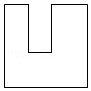
\includegraphics[width=0.2\textwidth]{./pics/Chapter_3/14.png}
    \end{figure}
    \vspace{1cm}
    % 2017年第二十二届“华罗庚金杯”少年数学邀请赛初赛试卷(小中组).doc; B
}

\item {
    {如图,在两张大小相同的大长方形纸片上,分别在角和边上各剪下一个大小相同的小正方形.若图\textcircled{2}阴影部分的周长比图\textcircled{1}阴影部分的周长多17厘米,那么剪下的小正方形周长为 \underline{\hbox to 10mm{}} 厘米.} \\
    \begin{figure}[H] 
        \centering
        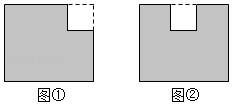
\includegraphics[width=0.4\textwidth]{./pics/Chapter_3/15.png}
    \end{figure}
    \vspace{1cm}
    % 华杯2017; 34
}


	\setbeamertemplate{background canvas}{
		
\includegraphics[width=\paperwidth,height=\paperheight]{./pics/end.jpg}
	}
	\begin{frame}
		\Huge{\centerline{下次课见}}
	\end{frame}
	%------------------------------------------------
	% \subsection{Subsection Example 2}
	
	% \begin{frame}
	% 	\frametitle{Bullet Points}
	% 	\begin{itemize}
	% 		\item What we do may be small, but it has a certain character of permanence.
	% 		\item Euclid geometry was as dazzling as first love.
	% 		\item Talk is cheap, solve the PDE.
	% 	\end{itemize}
	% \end{frame}
	
	% %------------------------------------------------
	
	% \begin{frame}
	% 	\frametitle{Blocks of Highlighted Text}
	% 	\begin{block}{Block 1}
	% 		Certainly the best times were when I was alone with mathematics: free of ambition and pretense, and indifferent to the world.
	% 	\end{block}
		
	% 	% \begin{block}{Block 2}
	% 	% 	Wir müssen wissen, Wir werden wissen.
	% 	% \end{block}
		
	% 	\begin{block}{Block 3}
	% 		If people do not believe that mathematics is simple, it is only because they do not realize how complicated life is.	
	% 	\end{block}
	% \end{frame}
	
	% %------------------------------------------------
	
	% \begin{frame}
	% 	\frametitle{Multiple Columns}
	% 	\begin{columns}[c] % The "c" option specifies centered vertical alignment while the "t" option is used for top vertical alignment
			
	% 		\column{.45\textwidth} % Left column and width
	% 		\textbf{Heading}
	% 		\begin{enumerate}
	% 			\item Statement
	% 			\item Explanation
	% 			\item Example
	% 		\end{enumerate}
			
	% 		\column{.5\textwidth} % Right column and width
	% 		Lorem ipsum dolor sit amet, consectetur adipiscing elit. Integer lectus nisl, ultricies in feugiat rutrum, porttitor sit amet augue. Aliquam ut tortor mauris. Sed volutpat ante purus, quis accumsan dolor.
			
	% 	\end{columns}
	% \end{frame}
	
	% %------------------------------------------------
	% \section{Second Section}
	% %------------------------------------------------
	
	% \begin{frame}
	% 	\frametitle{Table}
	% 	\begin{table}
	% 		\begin{tabular}{l l l}
	% 			\toprule
	% 			\textbf{Treatments} & \textbf{Response 1} & \textbf{Response 2}\\
	% 			\midrule
	% 			Treatment 1 & 0.0003262 & 0.562 \\
	% 			Treatment 2 & 0.0015681 & 0.910 \\
	% 			Treatment 3 & 0.0009271 & 0.296 \\
	% 			\bottomrule
	% 		\end{tabular}
	% 		\caption{Table caption}
	% 	\end{table}
	% \end{frame}
	
	% %------------------------------------------------
	
	% \begin{frame}
	% 	\frametitle{Theorem}
	% 	\begin{theorem}[Mass--energy equivalence]
	% 	\centerline{$E = mc^2$}
	% 	\end{theorem}
	% \end{frame}
	
	%------------------------------------------------
	
	% \begin{frame}[fragile] % Need to use the fragile option when verbatim is used in the slide
	% 	\frametitle{Verbatim}
	% 	\begin{example}[Theorem Slide Code]
	% 		\begin{verbatim}
	% 			\begin{frame}
	% 			\frametitle{Theorem}
	% 			\begin{theorem}[Mass--energy equivalence]
	% 			$E = mc^2$
	% 			\end{theorem}
	% 			\end{frame}
	% 		\end{verbatim}
	% 	\end{example}
	% \end{frame}

\end{document}
